
\section{Evaluation}\label{sec:evaluation}

In this section, we experimentally analyze various real-time aspects
of the DeepPicar. This includes
(1) measurement based worst-case execution time (WCET) analysis of
deep learning inferencing,
(2) the effect of using multiple cores in accelerating inferencing,
(3) the effect of co-scheduling multiple deep neural network models,
and 
(4) the effect of co-scheduling memory bandwidth intensive co-runners.

\subsection{Setup}

The Raspberry Pi 3 Model B platform used in DeepPicar equips a Boardcom
BCM2837 SoC, which has a quad-core ARM Cortex-A53 cluster,
running at up to 1.2GHz. Each core has 16K private I\&D caches, and all
cores share a 512KB L2 cache.
The chip also includes Broadcom's Videocore IV
GPU, although we did not use the GPU in our evaluation due to the lack
of sofware support (TensorFlow is not compatible with the Raspberry Pi's GPU).
For software, we use Ubuntu MATE 16.04, TensorFlow 1.1 and Python
2.7. We disabled DVFS (dynamic voltage frequency scaling) and
configured the clock speed of each core statically at the maximum 1.2GHz.

\subsection{Inference Timing for Real-Time Control}

For real-time control of a car (or any robot), the control loop
frequency must be sufficiently high so that the car can quickly
react to the changing environment and its internal states. In general,
control performance improves when the frequency is higher, though
computation time and the type of the particular physical system are
factors in determining a proper control loop frequency. While a standard
control system may be comprised of multiple control loops with
differing control frequencies---e.g., an inner control loop for lower-level
PD control, an outer loop for motion planning, etc.---DeepPicar's
control loop is a single layer, as shown earlier in
Figure~\ref{fig:controlloop}, since a single deep neural network
replaces the traditional multi-layer control pipline. (Refer to
Figure~\ref{fig:end-to-end-control} on the differences between the
standard robotics control vs. end-to-end deep learning approach).
This means that the DNN inference operation must be completed
within the inner-most control loop update frequency. To understand
achievable control-loop update frequencies, we experimentally measured
the execution times of DeepPicar's DNN inference operations.

% 50-200Hz for quadcopters:
% https://robotics.stackexchange.com/questions/231/what-frequency-does-my-quadcopter-output-sense-calculate-output-update-loop-need 
% https://quadmeup.com/pid-looptime-why-it-is-not-only-about-frequency/

\begin{figure}[t]
  \centering
  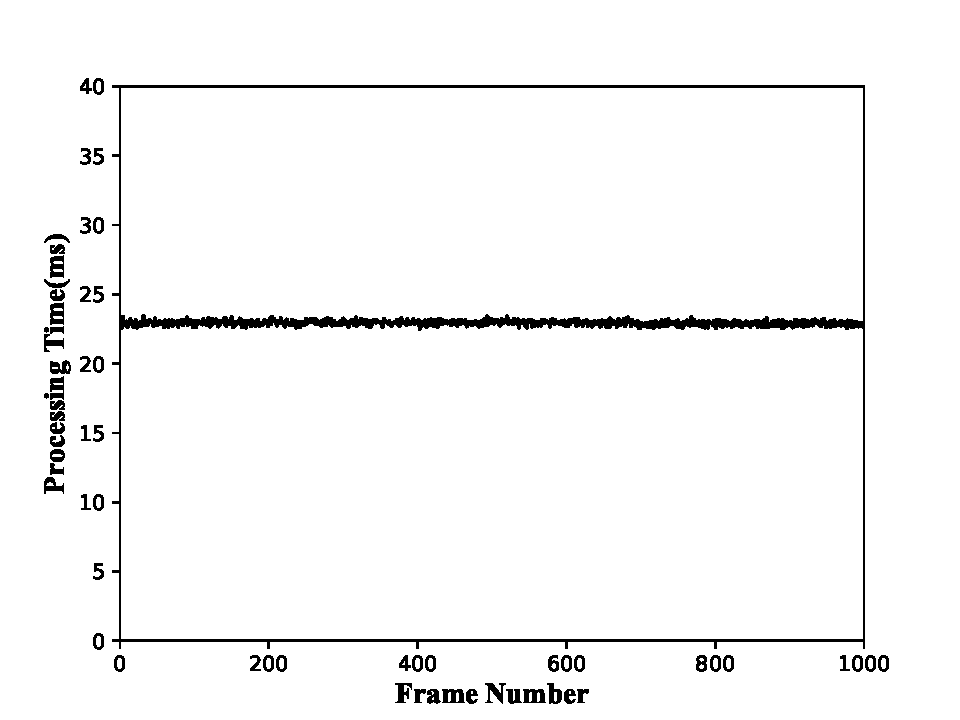
\includegraphics[width=.5\textwidth]{figs/Fig7_new}
  \caption{DeepPicar's control loop processing times over 1000 input image frames.}
  \label{fig:control-loop-timing}
\end{figure}

\begin{table}[t]
  \centering
  \begin{tabular} {| c | r | r | r | r |}
    \hline
    \textbf{Operation} & \textbf{Mean} & \textbf{Max} &   \textbf{99pct.} & \textbf{Stdev.} \\ \hline
    Image capture        & 2.28  &  4.94 &  4.54  & 0.52 \\ \hline
    Image pre-processing & 3.09  &  4.60 &  3.31  & 0.10 \\ \hline
    DNN inferencing      & 37.30 & 51.03 & 45.48  & 2.75 \\ \hline
    Total Time           & 42.67 & 56.37 & 50.70  & 2.80 \\ \hline
  \end{tabular}
  \caption{Control loop timing breakdown.}
  \label{tbl:control-loop-breakdown}
\end{table}

Figure~\ref{fig:control-loop-timing} shows the measured control loop 
processing times of the DeepPicar over 1000 image frames (one per each
control loop). We omit the first frame's processing time for cache
warmup. Table~\ref{tbl:control-loop-breakdown} shows the time
breakdown of each control loop. Note that all four CPU cores of the
Raspberry Pi 3 were used by the TensorFlow library when performing the
DNN inference operations.

First, as expected, we find that the inference operation
dominates the control loop execution time, accounting for about 85\% of
the execution time.
Second, and more importantly, we also find that the measured average
execution time of a single control loop is 42.67 ms, or 23.4 Hz and
the 99 percentile time is 50.70 ms.
This means that the DeepPicar can operate
at about a 20 Hz control frequency in real-time using only the on-board
Raspberry Pi 3 computing platform, as no remote computing resources 
were necessary. We consider these results respectable given the complexity
of the deep neural network, and the fact that the inference operation
performed by TensorFlow only utilizes the CPU cores of the
Raspberry Pi 3 (its GPU is not supported by Tensorflow).

In comparison, NVIDIA's DAVE-2 system, which has the exact same neural
network architecture, reportedly runs at 30 Hz~\cite{Bojarski2016}, which 
is just a bit faster than the DeepPicar. Although we believe it was not
limited by their computing platform (we will experimentally compare
performance differences among multiple embedded computing platforms,
including NVIDIA's Jetson TX2, later in
Section~\ref{sec:comparison}), the fact that the low-cost
Raspberry Pi 3 can achieve similar real-time control performance is
surprising.

\subsection{Effect of the Core Count to Inference Timing}

In this experiment, we investigate the scalability of performing
inference operations of DeepPicar's neural network with respect to the
number of cores. As noted earlier, the Raspberry Pi 3 platform has
four Cortex-A53 cores and TensorFlow 
provides a programmable mechanism to adjust how many cores are to be
used by the library. Leveraging this feature, we repeat the
same experiment described in the previous subsection with varying
numbers of CPU cores---from one to four.


\begin{figure}[h]
  \centering
  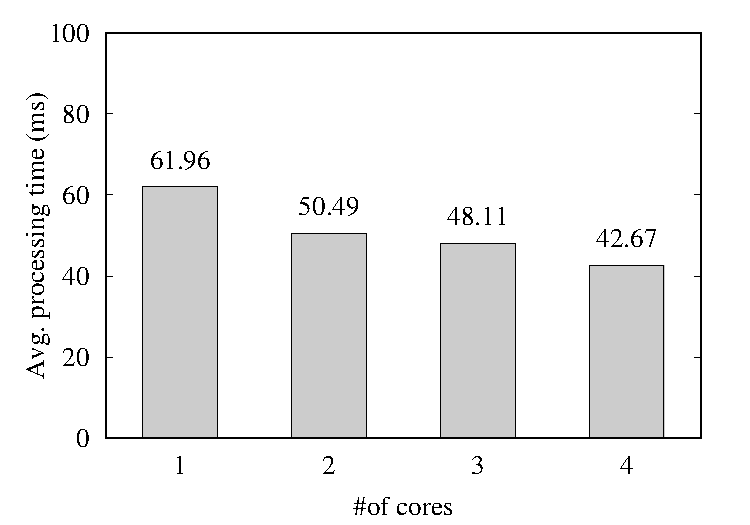
\includegraphics[width=.45\textwidth]{figs/perf_vs_corecnt}
  \caption{Average control loop execution time vs. \#of CPU
    cores.}
  \label{fig:perf-vs-corecnt}
\end{figure}

Figure~\ref{fig:perf-vs-corecnt} shows the average execution time of
the control loop as we vary the number of cores used by
TensorFlow. As expected, as we assign more cores, the average execution
time decreases---from 61.96 ms on a single core to 42.67 ms on four
cores (a 30\% improvement). However, the improvement is far from an ideal
linear scaling. In particular, from 2 cores to 3 cores, the
improvement is mere 2.38 ms (or 4\%). In short, we find that the
scalability of DeepPicar's deep neural network is not ideal on the
platform. We do not know whether it is due to the limitations of
TensorFlow's multicore implementation or if it's the model's inherent
characteristics. 

The poor scalability opens up the possibility of consolidating
multiple different tasks or different neural network models rather
than allocating all cores for a single neural network model. For
example, it is conceivable to use four cameras and four different
neural network models, each of which is trained separately and
executed on a single dedicated core. Assuming we use the same network
architecture for all models, then one might expect to achieve up to
15 Hz using one core (given 1 core can deliver 62 ms average
execution time). In the next experiment, we investigate the
feasibility of such a scenario.

\subsection{Effect of Co-scheduling Multiple DNN Models}

In this experiment, we launch multiple instances of DeepPicar's DNN
model at the same time and measure its impact on their inference
timings. In other words, we are interested in how shared resource
contention affects inference timing.

\begin{figure}[h]
  \centering
  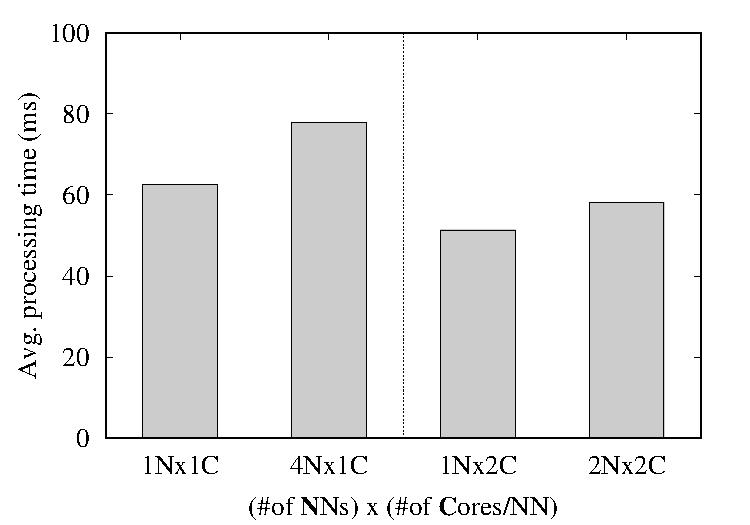
\includegraphics[width=.45\textwidth]{figs/perf_vs_modelcnt}
  \caption{Timing impact of co-scheduling multiple DNNs. 1Nx1C: one DNN
    model using one core; 4Nx1C: four DNN models each using one core;
    1Nx2C: one DNN model using two cores; 2Nx2C: two DNN models each
    using two cores.} 
  \label{fig:perf-vs-modelcnt}
\end{figure}

Figure~\ref{fig:perf-vs-modelcnt} shows the results. In the figure, the
X-axis shows the system configuration: \#of DNN models x \#of CPU
cores/DNN. For example, '4Nx1C' means running four DNN models each of
which is assigned to run on one CPU core, whereas '2Nx2C' means running
two DNN models, each of which is assigned to run on two CPU
cores. The Y-axis shows the average inference timing.
The two bars on the left show the impact of co-scheduling four DNN
models. Compared to executing a single DNN model on one CPU core
(1Nx1C), when four DNN models are co-scheduled (4Nx1C), each model
suffers an average inference time increase of approximately 15 ms,
$\sim$24\%. On the other hand, when two DNN models, each using two CPU
cores, are co-scheduled (2Nx2C), the average inference timing is increased by
about 7 ms, or 10\%, compared to the baseline of running one model
using two CPU cores (1Nx2C). 

\begin{figure}[h]
  \centering
  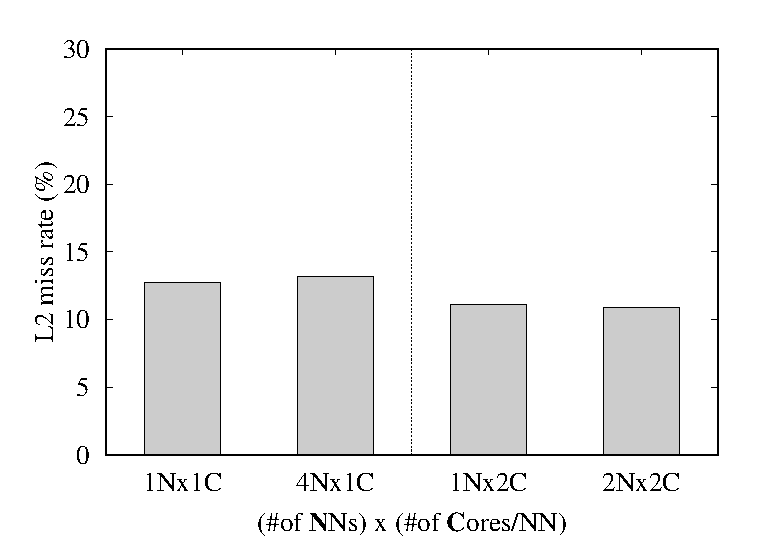
\includegraphics[width=.45\textwidth]{figs/l2missrate_vs_modelcnt}
  \caption{L2 cache miss rates of different neural network and core
    assignments. X-axis is the same as Figure~\ref{fig:perf-vs-modelcnt}.} 
  \label{fig:l2missrate-vs-modelcnt}
\end{figure}

These increases in inference times in the co-scheduled scenarios are
expected and likely caused by contention in the shared hardware
resources, such as the shared L2 cache and/or the DRAM controller.
To further analyze the source of contention, we use hardware
performance counters of the processor. Specifically, we measure L2
miss rates of the DNN models first in isolation and then after
co-scheduling other models. If the shared L2 cache is the primary
source of inteference, then the measured L2 miss rates will
increase. Figure~\ref{fig:l2missrate-vs-modelcnt} shows the results.
As can be see in the figure, L2 miss rates are largely unchanged
regardless of whether multiple models are co-scheduled or not. This
suggests that the shared L2 cache is not the bottleneck that caused
execution time increases. In other words, DNN models don't appear to be
sensitive to the shared L2 cache space. % L2 partitioning is probably
                                % not going to be useful.
Instead, we hypothesize that it is likely caused by the memory
controller---the only other major shared hardware source---where
memory requests from different CPU cores contend, which would result
in increased memory access latency. While some Intel processors
provide incore hardware counters that can measure average memory
access latency~\cite{ye2016maracas}, we were not able to identify
whether such hardware counters exist in the BCM2837 processor of
Raspberry Pi 3 due to the lack of documentation. Instead, in the next
experiment, we use memory intensive synthetic benchmarks to test the
hypothesis.

\subsection{Effect of Co-scheduling Memory Performance Hogs}\label{sec:eval-memhog}

In order to determine how contended DRAM requests affect the DNN
inference timing of the DeepPicar, we use a synthetic memory
intensive benchmark from the IsolBench suite~\cite{Valsan2016}.

We run a single DNN model one core, and
co-schedule an increasing number of the memory intensive synthetic
benchmarks~\footnote{We use the \emph{Bandwidth} benchmark in the
  IsolBench suite, with the following command line parameters: \texttt{\$
  bandwdith -a write -m 16384}}, on the remaining idle cores.

\begin{figure}[h]
  \centering
  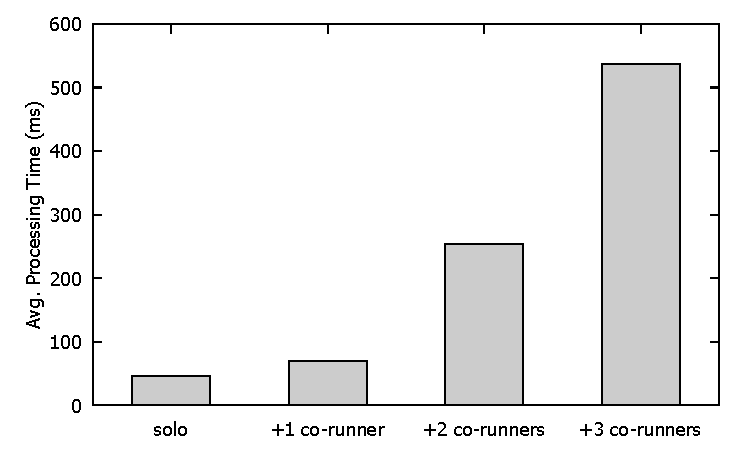
\includegraphics[width=.45\textwidth]{figs/perf_vs_bandwidth}
  \caption{Effect of memory performance hogs on the DNN
    inferencing. The DNN model uses Core 0 and memory-hog co-runners
    use the rest of the cores.}
  \label{fig:}
\end{figure}

Figure~\ref{fig:} shows the normalized execution time and L2 miss-rate
of the DNN model running on the Core 0 as a function of the number of
co-scheduled memory intensive synthetic benchmarks. First, as we
increase the number of co-runners, the DNN model's execution times are
increased---by up to 9.6X---even though the DNN model is running on a
dedicated core (Core 0). On the other hand, the DNN model's L2
cache-miss rates do not increase as much. This suggests that
the DNN model's exeuction increase cannot be fully explained by
increases in L2 cache-misses. Instead, as we hypothesized in the previous
experiment, the increased memory pressure from the co-scheduled memory
intensive benchmarks is likely the primary cause of the DNN model's execution
time increase. Therefore, we conclude that DeepPicar's DNN model is
more senstive to DRAM access latency than L2 cache space.

This observation suggests that shared cache partitioning
techniques~\cite{Gracioli2015,Kim2016} may not be effective isolation
solutions for DeepPicar, as its AI workload is more sensitive to memory
performance. Instead, memory controller focused isolation solutions,
either hardware or software-based ones (e.g.,~\cite{Guo2017,Yun2013}),
may be more important. Although our observation is made on a single
hardware platform running on a single DNN workload, we suspect that
many AI workloads may exhibit similar characteristics.

\begin{table*}[h]
  \centering
  \begin{tabular}{|c|c|c|c|}
    \hline
    Item    & Raspberry Pi 3 (B)   & Intel UP                  & NVIDIA Jetson TX2\\
    \hline
            & BCM2837              & X5-Z8350 (Cherry Trail)   & Tegra X2 \\
    CPU     & 4x Cortex-A53@1.2GHz/512KB L2  &
              4x Atom@1.92GHz/2MB L2 &
              4x Cortex-A57@2GHz/2MB L2 \\
            &              &              & 2x Denver@2.0GHz/2MB L2 (not used)  \\
    \hline
    GPU     &  VideoCore IV (not used)    &
               Intel HD 400 Graphics (not used) &
               Pascal 256 CUDA cores   \\
    \hline
    Memory  & 1GB LPDDR2   &  2GB DDR3L     & 8GB LPDDR4              \\
    \hline
  \end{tabular}
  \caption{Compared embedded computing platforms}
  \label{tbl:platforms}
\end{table*}

\subsection{Summary of the Findings}
So far, we have evaluated DeepPicar's real-time
characteristics from the perspective of end-to-end deep learning based
real-time control, and made several observations.

First, we find that DeepPicar's computing platform,
the Raspberry Pi 3 Model B, offers adquate computing capacity to
perform real-time control of the RC car at 20 Hz frequency (or
50ms per control loop). Given the complexity of the DNN used, we
were pleasantly suprised by this finding. The time breakdown shows that
the DNN inferencing operation, performed by the Tensorflow library,
dominates the execution time, which is expected.

Second, we find that scalability of Tensorflow's DNN 
implementation is limited. We find that using all four cores is 
only about 30\% better than using just a single core.

Third, we find that consolidating multiple DNN models---on different CPU
cores---is feasible as we find: (1) DNN performance using a single
core is not much worse than using multiple cores; (2) multiple DNN
models running simultaneously do not cause severe interference with
each other.

Lastly, we find that consolidating memory (DRAM) performance
intensive applications could jeopadize DNN performance, because DNN
performance appears to be very sensitive to memory performance; we observe up
to 9.6X slowdown in DNN performance by co-scheduling synthetic memory 
bandwidth intensive applications on idle cores.